\documentclass[a4paper]{article}

  \usepackage{fullpage} % Package to use full page
  \usepackage{parskip} % Package to tweak paragraph skipping
  \usepackage{tikz} % Package for drawing
  \usepackage{amsmath}
  \usepackage{siunitx}
  \usepackage{amsfonts}
  \usepackage{amssymb}
  \usepackage{hyperref}
  \usepackage[utf8]{inputenc}
  \usepackage[english]{babel}
  \usepackage{multicol}
  \usepackage{graphicx}
  \graphicspath{ {./images/} }
  
  \newcommand\tab[1][0.5cm]{\hspace*{#1}}
  
  \title{Laboratory 6: Introduction to the Use of PSPICE}
  \author{Adrian Darian}
  \date{11/4/2020}
  
  \begin{document}
  
\maketitle
  
\section*{Objectives}
• Learn what PSPICE is and its basic functions. \\
• Learn how to use PSPICE to construct a simple circuit. \\
• Learn how to use PSPICE to simulate and analyze the circuit. \\

\section*{Equipment and components}
• A computer \\
• PSPICE software \\

\section*{Preliminary}
PSPICE is a PC version of SPICE which runs on personal computers and offers many improvements over SPICE. SPICE is an acronym for Simulation Program with Integrated Circuit Emphasis. PSPICE is widely used in industries and universities. Though developed for IC design, it can be a useful tool for both the student and practicing circuit designer with many non-IC circuits. The version of PSPICE for use in the School of Engineering lab (SRE 303) is a PSPICE Student V.9.1. You can download the updated free trial version 17.4 from https://www.orcad.com/resources/orcaddownloads or the updated student 17.4 from https://www.orcad.com/orcad-academic-program. You can also download the newest version of MacSpice from https://www.macspice.com/Download.html for mac computers. You can refer to the link http://www.macspice.com/ for how to use MacSpice.

\section*{Procedure Version 17.4}
\begin{itemize}
  \item[1.] The following circuit will be built and simulated in PSPICE. You can observe steady-state responses of a RC circuit. The input (source) is a sinusoidal input and the output(response) is the voltage across the capacitor. \\
  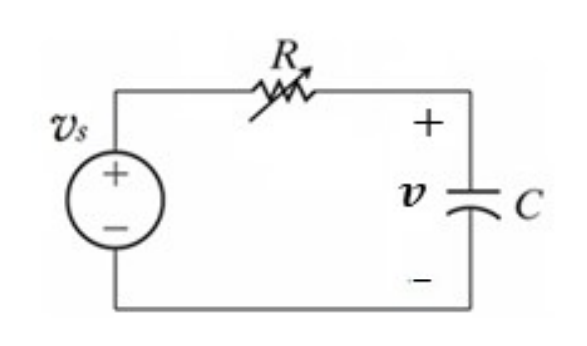
\includegraphics[scale=0.5]{diagram.png} \\   
  \item[2.] Go to the All Program. Under the "OrCad Trial 17.4", click the "Capture CIS 17.4" and the window "OrCAD Capture" opens. \\
  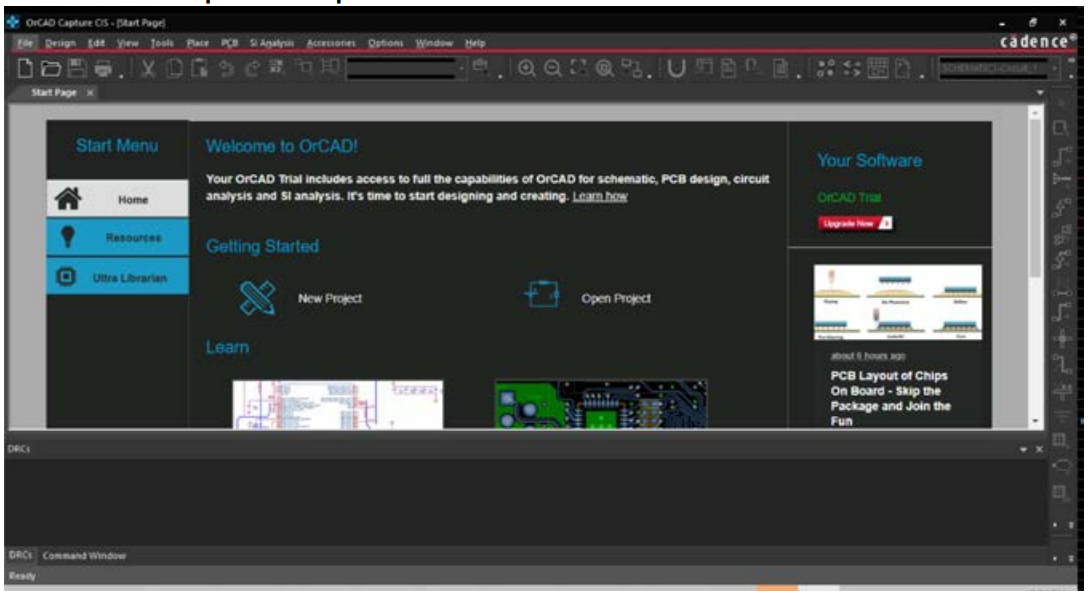
\includegraphics[scale=0.5]{1.png} \\ 
  \item[3.] Click the "Create Document" icon on the tool bar and create a name for your design on the desktop of your computer.
  \begin{itemize}
    \item[a.] Make sure to check "Enable PSpice Simulation" dialog box as shown below.
    \item[b.] Select a location for the New Project. Then press OK. \\
    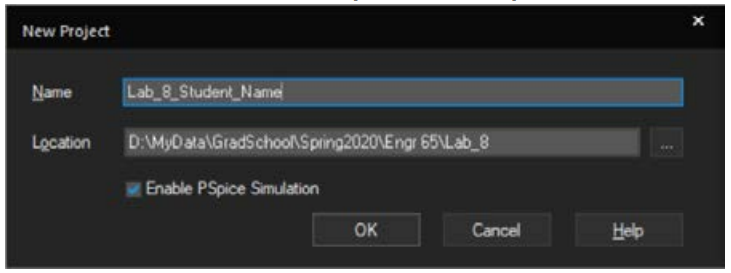
\includegraphics[scale=0.5]{2.png} \\ 
    \item[c.] Select "Create based upon existing project" and choose "AnalogGNDSymbol.opj". Then press OK. \\
    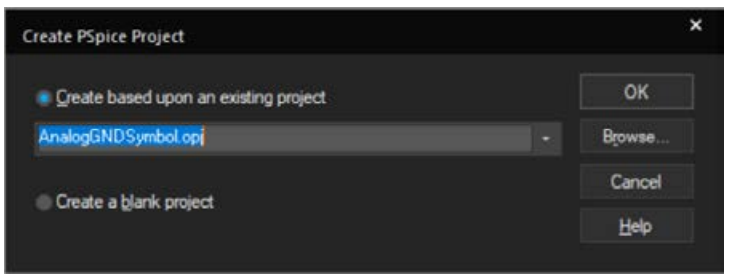
\includegraphics[scale=0.5]{3.png} \\ 
    \item[d.] Next, locate the left menu called "Analog or Mixed A/D". Expand "Design Resources" > ".\\lab\_$8$\_student\_name" > "Schematic$1$" and double click on "PAGE$1$". \\
    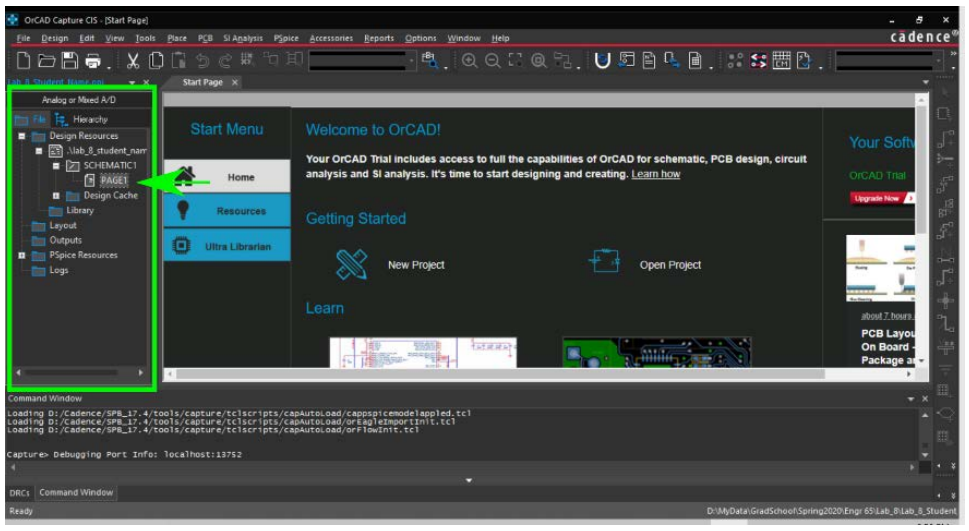
\includegraphics[scale=0.5]{4.png} \\ 
    \item[e.] Your screen should look like the image below. \\
    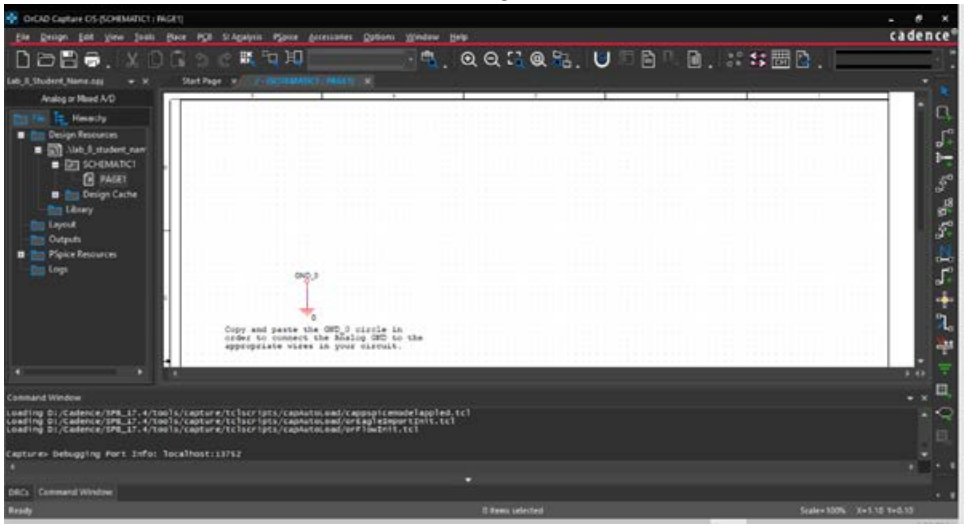
\includegraphics[scale=0.5]{5.png} \\ 
  \end{itemize} 
  \item[4.] On the right of the window, locate the tool bar menu.
  \begin{itemize}
    \item[a.] Find following symbol that is highlighted in green (see image to the right). This is the add "part" tool. When clicked, a new menu will appear that allows you to search for circuit elements. You can use the shortcut key by pressing "P".
    \item[b.] Find the symbol highlighted in red (see image to the right). This is the add "wire" tool. This tool allows you to connect the elements of your circuit. You can also use the shortcut key "W".
    \item[c.] Now click on the add "part" symbol or press "P" to bring up the "Place Part" menu.
  \end{itemize} 
  \item[5.] Below is the "Place Parts" Menu. If you do not have any libraries in the "Libraries", Click "Add Library" and under "Pspice" directory, select all and then click "Open". Now you are ready to build a circuit. \\
  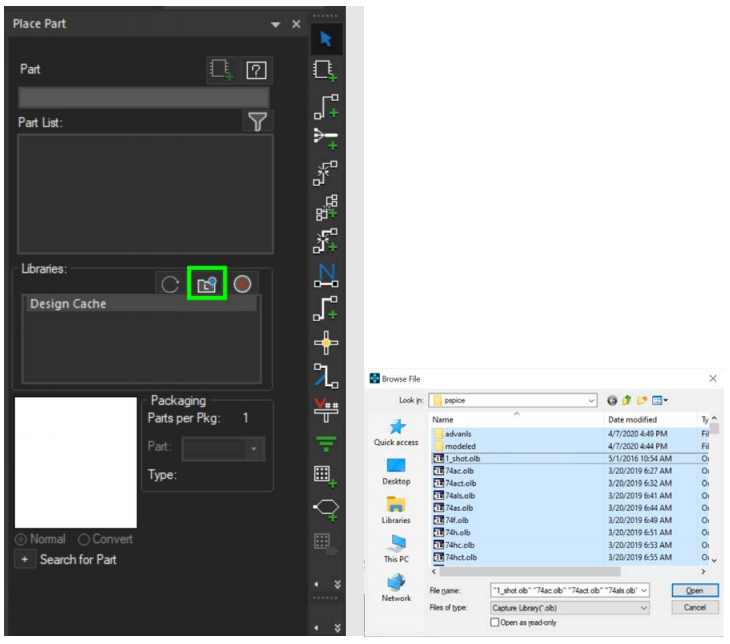
\includegraphics[scale=0.5]{6.png} \\ 
  \item[6.] Build the following the circuit by selecting different parts from the window.
  \begin{itemize}
    \item[a.] In the search field, type "R/Analog".
    \begin{itemize}
      \item[i.] Then click on "R/Analog" in the Parts List.
      \item[ii.] Next click the "Place Part" symbol that is right above the search field or use the shortcut key "Enter". This changed the mouse pointer to the part you choose.
      \item[iii.] On the schematic page, left click where you would like to place the part.
      \item[iv.] Press "Esc" to stop adding parts. Note: If you add to many parts, after pressing the "Esc" key, you can left click on the part then push "backspace" to delete the extra part.
      \item[v.] You can change the value of the part by double clicking on the part to enter the Property Editor. For a resistor, you must scroll all the way to the right of the description. Ensure the resistor’s value is \SI{1}{\kilo\ohm}.
      \item[vi.] You can rotate the part by right clicking on the element and selecting rotate. \\
      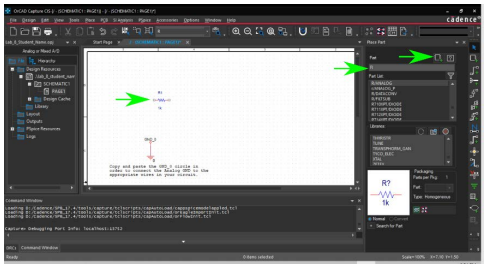
\includegraphics[scale=0.5]{7.png} \\ 
    \end{itemize} 
  \item[b.] Repeat the same procedure but search for "C".
  \begin{itemize}
    \item[i.] Type "C" in the "Part" search field.
    \item[ii.] Press "Enter’ to place a capacitor on the schematic.
    \item[iii.] Press "Esc" to stop adding new parts.
    \item[iv.] Double click with the left mouse button to bring up the Property Editor Menu.
    \item[v.] Scroll to the right and find the "value" field and set the capacitance of the capacitor as $\SI{1}{\mu}F$ by typing in "1u". Then click on apply. Close the Property Editor.
    \item[vi.] \\
    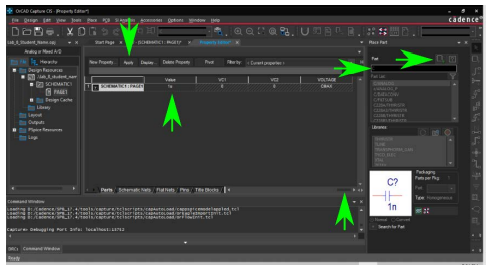
\includegraphics[scale=0.5]{8.png} \\ 
  \end{itemize} 
  \item[c.] Repeat the same procedure but search for "Vsin"
  \begin{itemize}
    \item[i.] Select "Vsin" from the parts menu and press "Enter" to and the part.
    \item[ii.] Press "Esc" to stop placing new parts.
    \item[iii.] Double click with the left mouse button on the Source to open the Property Editor.
    \item[iv.] Scroll to the right to find the value fields and set them to "FREQ=100", "VAMPL=10" and "VOFF=0". Note: These fields are not all next to each other. You will have to scroll all the way to the right to find the last two value fields. See images below.
  \end{itemize}
  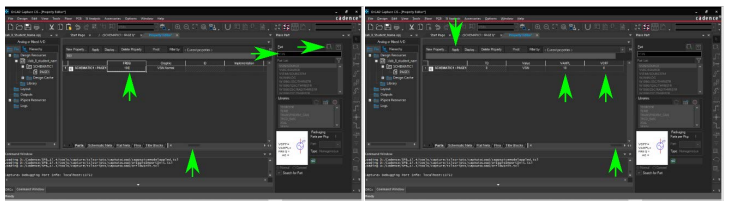
\includegraphics[scale=0.5]{9.png} \\
  \item[d.] If your schematic is missing the "Ground" icon, repeat the same procedure to search for "0" and select the item from the parts list. At this point your schematic show look like the image below. \\
  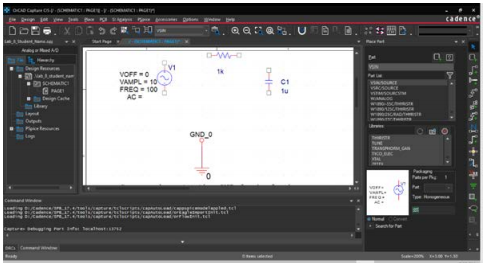
\includegraphics[scale=0.5]{10.png} \\ 
  \item[e.] Locate the add wire symbol on the right menu bar or press "W". This enables you to add a connecting wire to all you join all your elements together.
  \begin{itemize}
    \item[i.] Note: Most problems stem from the ground not being connected to the circuit wire. It is easier to delete the "GND\_0" text, wire from the ground and the "o" symbol. Then connect a wire from the square in the ground to the circuit until you see it connect properly. See the pink dot.
  \end{itemize}
  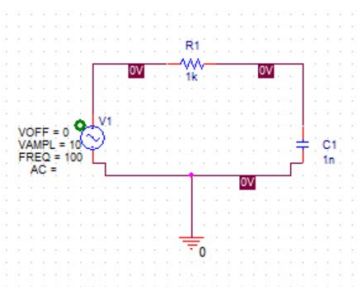
\includegraphics[scale=0.5]{11.png} \\
  \end{itemize} 
  \item[7.] Please note $vs$ is a sinusoidal voltage source with the expression of $vs = V_{s}sin\si{\omega}t = 10sin\SI{200}{\pi}t$ , $v$ is the output across the capacitor and $v = V_{m}sin(\si{\omega} + \si{\varphi})$. Note: $V_{m}$ and $V_{s}$ are the peak value of the output voltage and voltage source, respectively, and $\si{\varphi}$ is called the phase angle. Here, $\si{\varphi}$ also represents the phase angle difference between two voltages: $vs$ and $v$.
  \item[8.] To add a Voltage Measurement, click on the "PSpice" in the top menu.
  \begin{itemize}
    \item[a.] Next, find "Markers" then select the first option "Voltage Level" \\
    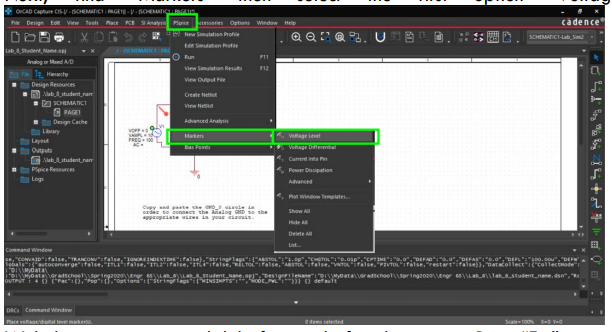
\includegraphics[scale=0.5]{12.png} \\ 
    \item[b.] With the mouse pointer, click before and after the resistor. Press "Esc" to exit voltage marker mode. \\
    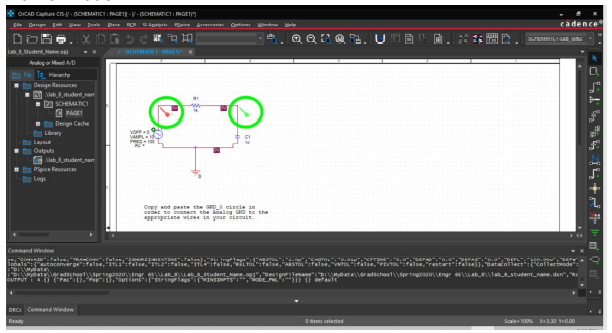
\includegraphics[scale=0.5]{13.png} \\ 
  \end{itemize} 
  \item[9.] In the PSpice menu select new simulation
  \begin{itemize}
    \item[a.] Name your simulation. Then click create. \\
    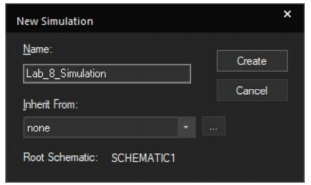
\includegraphics[scale=0.5]{14.png} \\ 
    \item[b.] You will see the Simulation Settings window.
    \begin{itemize}
      \item[i.] In the Analysis tab, change Analysis Type to "Time Domain (Transient)".
      \item[ii.] Change "Run to Time" to "10ms".
      \item[iii.] Leave "Start saving data after" value as zero.
      \item[iv.] In the "Transient Options" section, change "Maximum Step Size" to "5us" \\
      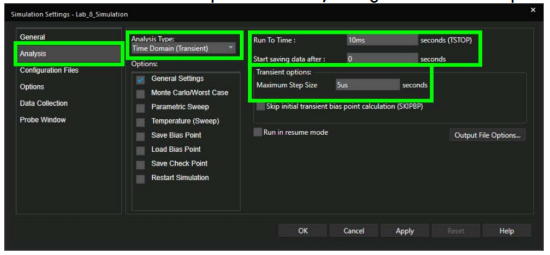
\includegraphics[scale=0.5]{15.png} \\ 
      \item[v.] Next click on the "Data Collection" Tab.
      \item[vi.] Change Voltages to "At Markers Only". Change Current, Power and Noise to "None" \\
      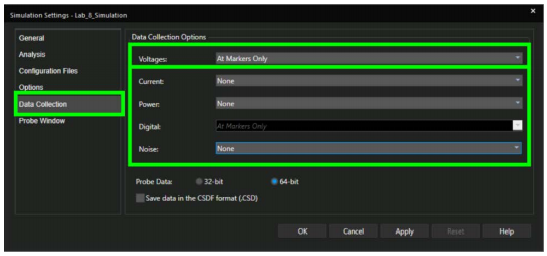
\includegraphics[scale=0.5]{16.png} \\ 
      \item[vii.] Next click Apply then OK.
    \end{itemize} 
  \end{itemize} 
  \item[10.] In the PSpice menu, find and click on run. This will open the simulation window. As seen below. \\
  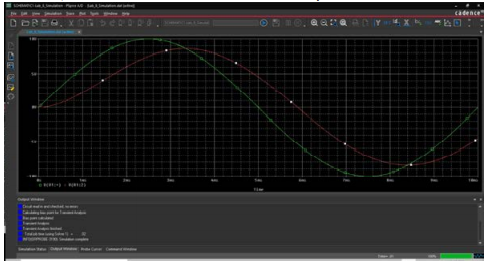
\includegraphics[scale=0.5]{17.png} \\ 
  \item[11.] Fill up the tables below for the first cycle and third cycle (increase the simulation time if needed) of $vm$, $vs$ $\si{\varphi}$ and plot $V_{m}$ and $\si{\varphi}$ in terms of $R$. For a given $R$, are $vm$, $vs$ $\si{\varphi}$ same in the different cycles? Do not need to explain. 
\end{itemize}

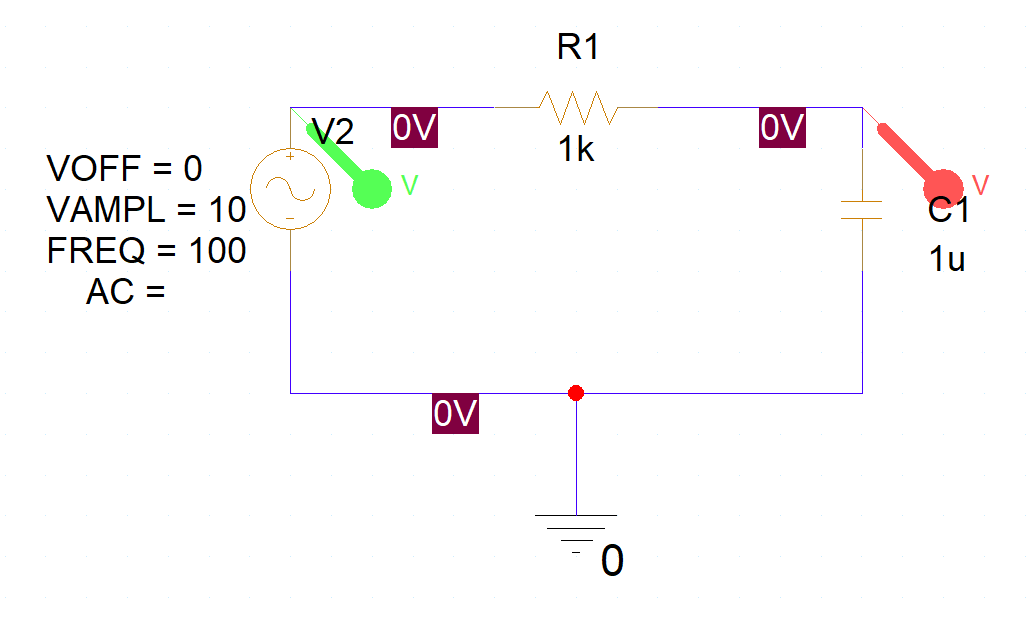
\includegraphics[scale=0.5]{circuit.png} \\

\section*{Capacitive responses in the RC circuit (the First Cycle)}
\begin{tabular}{|c|c|c|c|c|c|c|c|c|c|c|}
\hline
$R(\si{\ohm})$ & 50 & 100 & 200 & 500 & 1000 & 1500 & 2000 & 2500 & 3000 & 4000 \\
\hline
$V_{m}$ & 9.99507 & 9.98032 & 9.92197 & 9.54762 & 8.62234 & 7.71487 & 6.93512 & 7.71487 & 5.73226 & 4.87072 \\
\hline
$V_{sm}$ & 10 & 10 & 10 & 10 & 10 & 10 & 10 & 10 & 10 & 10 \\
\hline
$\si{\varphi}$ & 0.00493 & 0.01968 & 0.07803 & 0.45238 & 1.37766 & 2.28513 & 3.06488 & 2.28513 & 4.26774 & 5.12928 \\
\hline
\end{tabular}

\section*{Capacitive responses in the RC circuit (the Third Cycle)}
\begin{tabular}{|c|c|c|c|c|c|c|c|c|c|c|}
\hline
$R(\si{\ohm})$ & 50 & 100 & 200 & 500 & 1000 & 1500 & 2000 & 2500 & 3000 & 4000 \\
\hline
$V_{m}$ & 9.99507 & 9.98032 & 9.92197 & 9.54762 & 8.62234 & 7.71487 & 6.93512 & 6.28121 & 5.73226 & 4.87072 \\
\hline
$V_{sm}$ & 10 & 10 & 10 & 10 & 10 & 10 & 10 & 10 & 10 & 10 \\
\hline
$\si{\varphi}$ & 0.00493 & 0.01968 & 0.07803 & 0.45238 & 1.37766 & 2.28513 & 3.06488 & 3.71879 & 4.26774 & 5.12928 \\
\hline
\end{tabular}

\section*{Questions and Conclusions}
• Are there any frequency differences between the source (input) and the response (output)? \\
Yes, there are frequencies between the input and the output. As the resistance increases the response and phase shift also increase. \\
• Are there any changes in peak value of the source and the response when you change the resistance of the resistor? \\
Yes, the peak value sources do not change as the resistance chances. \\
• Are there any changes in the phase $\si{\varphi}$ in the response? \\
Yes, there are changes in the phase as the resistor changes: as you raise the resistance the shift is also increased. \\
• Summarize your findings of this lab. \\
I found that as I increased the resistance the $V_{m}$ would decrease, increasing the $\si{\varphi}$ value. However, the $V_{sm}$ remained the same value the whole time. I also found out that in the PSPICE simulation you can make expressions to mimic the expression of the circuit and display the correct values.

\end{document}